
\begin{figure*}[t]
\centering
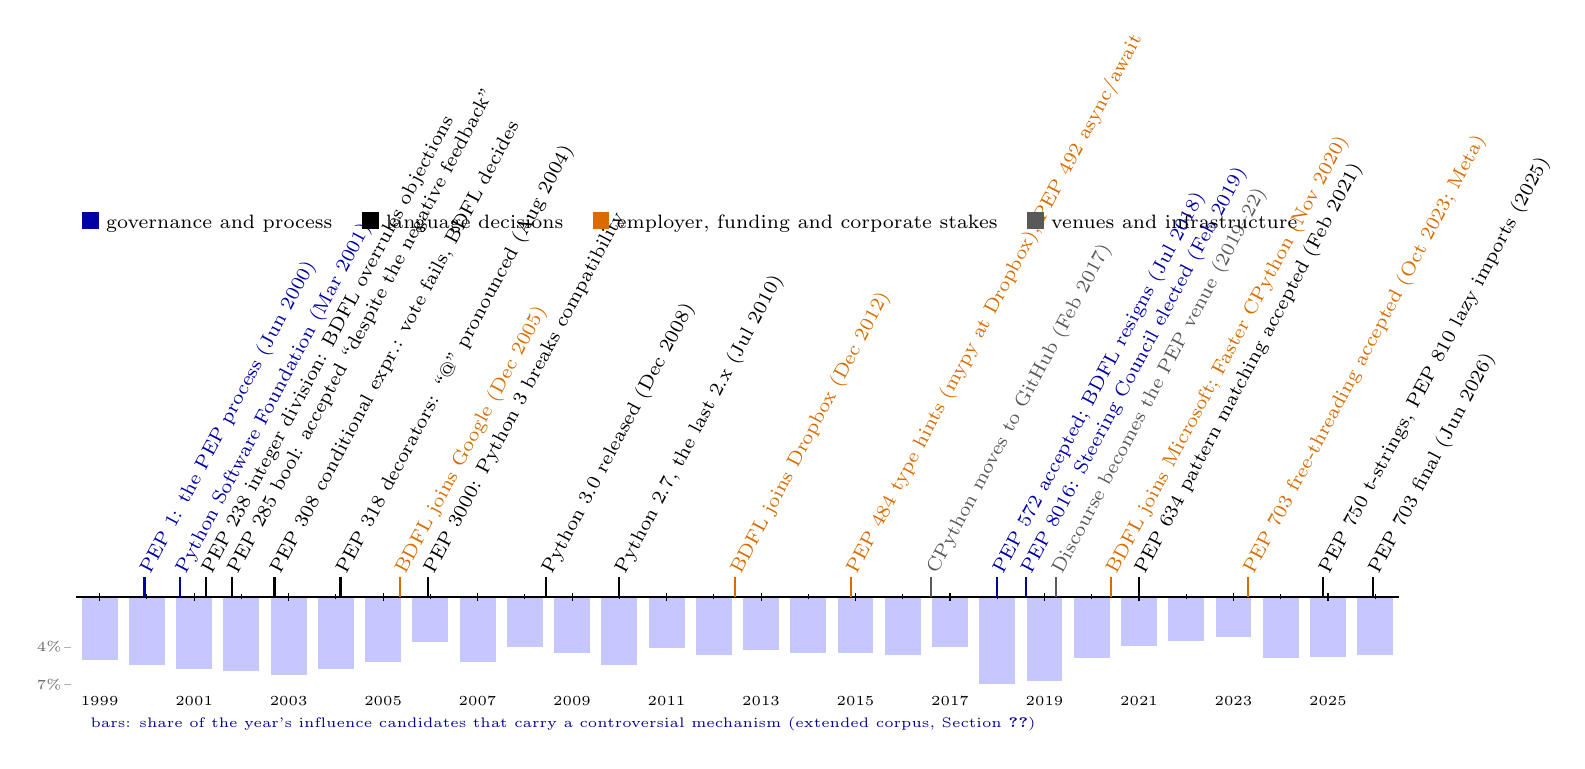
\begin{tikzpicture}[x=0.6cm, y=1cm, font=\scriptsize]
  % ---- yearly share of influence candidates that carry a controversial mechanism (extended corpus) ----
  \foreach \yr/\p in {1999/5.0, 2000/5.4, 2001/5.7, 2002/5.9, 2003/6.2, 2004/5.7, 2005/5.2, 2006/3.6, 2007/5.2,
                      2008/4.0, 2009/4.5, 2010/5.4, 2011/4.1, 2012/4.6, 2013/4.2, 2014/4.5, 2015/4.5, 2016/4.6,
                      2017/4.0, 2018/6.9, 2019/6.7, 2020/4.9, 2021/3.9, 2022/3.5, 2023/3.2, 2024/4.9, 2025/4.8, 2026/4.6} {
    \pgfmathsetmacro{\xl}{\yr-1999+0.12}
    \pgfmathsetmacro{\xr}{\yr-1999+0.88}
    \pgfmathsetmacro{\h}{-\p*0.16}
    \fill[blue!22] (\xl,0) rectangle (\xr,\h);
  }
  \draw[gray!60] (-0.25,-0.64) -- (-0.1,-0.64) node[left, text=gray!80!black, font=\tiny] {4\%};
  \draw[gray!60] (-0.25,-1.12) -- (-0.1,-1.12) node[left, text=gray!80!black, font=\tiny] {7\%};
  \node[anchor=west, text=blue!60!black, font=\tiny] at (0.1,-1.62) {bars: share of the year's influence candidates that carry a controversial mechanism (extended corpus, Section~\ref{sec:rq6})};
  % ---- axis and years ----
  \draw[thick] (0,0) -- (28,0);
  \foreach \yr in {1999,2001,...,2025} {
    \draw (\yr-1999+0.5,0.05) -- (\yr-1999+0.5,-0.05);
    \node[font=\tiny] at (\yr-1999+0.5,-1.33) {\yr};
  }
  \foreach \yr in {2000,2002,...,2026} { \draw (\yr-1999+0.5,0.03) -- (\yr-1999+0.5,-0.03); }
  % ---- landmark influences: x = fractional year, colour = kind ----
  \tikzset{gov/.style={blue!65!black}, lang/.style={black}, venue/.style={gray!70!black}, corp/.style={orange!85!black}}
  \foreach \x/\c/\t in {
    2000.45/gov/{PEP 1: the PEP process (Jun 2000)},
    2001.2/gov/{Python Software Foundation (Mar 2001)},
    2001.75/lang/{PEP 238 integer division: BDFL overrules objections},
    2002.3/lang/{PEP 285 bool: accepted ``despite the negative feedback''},
    2003.2/lang/{PEP 308 conditional expr.: vote fails, BDFL decides},
    2004.6/lang/{PEP 318 decorators: ``@'' pronounced (Aug 2004)},
    2005.85/corp/{BDFL joins Google (Dec 2005)},
    2006.45/lang/{PEP 3000: Python 3 breaks compatibility},
    2008.95/lang/{Python 3.0 released (Dec 2008)},
    2010.5/lang/{Python 2.7, the last 2.x (Jul 2010)},
    2012.95/corp/{BDFL joins Dropbox (Dec 2012)},
    2015.4/corp/{PEP 484 type hints (mypy at Dropbox), PEP 492 async/await},
    2017.1/venue/{CPython moves to GitHub (Feb 2017)},
    2018.5/gov/{PEP 572 accepted; BDFL resigns (Jul 2018)},
    2019.1/gov/{PEP 8016: Steering Council elected (Feb 2019)},
    2019.75/venue/{Discourse becomes the PEP venue (2019--22)},
    2020.9/corp/{BDFL joins Microsoft; Faster CPython (Nov 2020)},
    2021.5/lang/{PEP 634 pattern matching accepted (Feb 2021)},
    2023.8/corp/{PEP 703 free-threading accepted (Oct 2023; Meta)},
    2025.4/lang/{PEP 750 t-strings, PEP 810 lazy imports (2025)},
    2026.45/lang/{PEP 703 final (Jun 2026)}} {
    \draw[\c, thick] (\x-1999,0) -- (\x-1999,0.25);
    \node[\c, rotate=62, anchor=west, inner sep=1pt] at (\x-1999,0.27) {\t};
  }
  % ---- legend ----
  \node[anchor=south west, align=left, font=\scriptsize, inner sep=2pt] at (0,4.55) {%
    \textcolor{blue!65!black}{\rule{6pt}{6pt}} governance and process \quad
    \textcolor{black}{\rule{6pt}{6pt}} language decisions \quad
    \textcolor{orange!85!black}{\rule{6pt}{6pt}} employer, funding and corporate stakes \quad
    \textcolor{gray!70!black}{\rule{6pt}{6pt}} venues and infrastructure};
\end{tikzpicture}
\caption{Landmark influences on the Python project from the start of the corpus (python-dev, May 1999) to September 2026, above a corpus-derived measure of contestation: the share of each year's influence candidates that carry one of the seven controversial mechanisms (Section~\ref{sec:rq6}). Dates are from PEP headers, the \texttt{python/peps} history and python.org. Events were chosen because they changed who decides (governance), what the language is (each is the year's most discussed PEP in the corpus), who pays for the work, or where the discussion happens. The most contested years are 2003 (PEP~308's failed vote) and 2018--2019 (PEP~572 and the governance transition); the Steering Council's first years (2021--2023) are the least contested in the corpus.}
\label{fig:timeline}
\Description{A horizontal timeline from 1999 to 2026 with twenty-one labelled, colour-coded events rising from the axis at an angle, and a bar chart below the axis showing the yearly percentage of controversial influence candidates, peaking at about seven percent in 2018.}
\end{figure*}
